\subsection{Level Story}

The sun is setting, and a storm is raging: the perfect climate to complete the Animagus ritual. Minerva and Delphini had reached the Forbidden Forest, a peaceful and isolated enough place for that purpose. Minerva casts the final spell, pronouncing increasingly loudly "Amato Animo Animato Animagus", with the wand pointing at her heart. Finally, Minerva drinks the potion.

\begin{figure}[H]
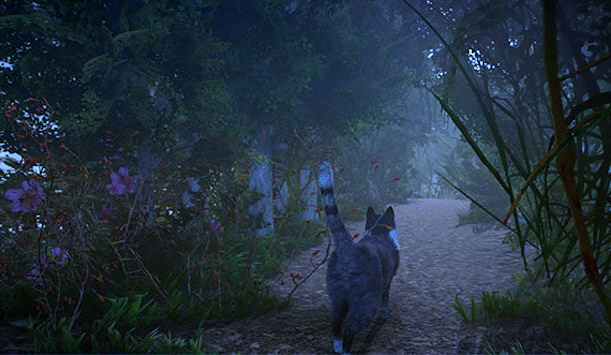
\includegraphics[max width=\textwidth]{../Pictures/Level/Script/Minerva_cat_picture.jpg}
\end{figure} 

\begin{dialogue}{Dialogue 1}
	\speak{Delphini}{I can't believe it! It really worked!}
	\speak{Minerva}{*Meow*...}
	\speak{Delphini}{Aww... would you look at this cute cat! I guess I've never seen this "soft side" of yours, Minerva.}
\end{dialogue} 

Delphini outbursts in laughter, and looks at Minerva trying to get used to her new shape. She tries climbing on trees, jumping around the forest, to finally come back in her human form. \\

\pagebreak

\begin{dialogue}{Dialogue 2}
	\speak{Delphini}{Alright then, what does it feel like to be a furball?}
	\speak{Minerva}{Oh come on! \*laughs\* If *anything*, as a cat I won't be forced to reply at your nonsensical provocations.}
	\speak{Delphini}{As if, I'm fully aware you can't live without my Irish irony; and you know that too.}
	\speak{Minerva}{You'd be surprised... Anyways, it's getting late, we should head back to the castle before it's night-time.}
\end{dialogue} 

The girls follow the path that goes back to the castle, until as they're about to leave the borders of the Forest, they're ambushed by a vicious three-headed dog, a Cerberus!\\

\fullwidthgraphics{../Pictures/Level/Script/Cerberus_picture.jpg}

Quickly Minerva and Delphini prepare to fight it, wand in hand. Minerva tries to make her best use of spells and transfigurations, while Delphini tries to combine her spells with Minerva's. While fighting, Delphini suddenly remembers the weak point of the three-headed dog: a particular melody can be played in order to put the beast to sleep, making quick work of it.

In the end, they manage to defeat the Cerberus, either by putting it to sleep or by making him faint with other spells; the battle, however, took longer than expected: it's too late to get back in the Castle through the main gate, as the students are expected to not leave it during the night.

They rush up to the back entrance of the castle, where they discuss a plan to proceed without being caught by the caretaker or by the prefects.\\
  
\begin{dialogue}{Dialogue 3} 
	\speak{Minerva}{It's too late! It's already closed!}
	\speak{Delphini}{As if we didn't know it! Move, I'll show you how it's done!}
\end{dialogue}

Delphini tries to cast the Alohomora spell, but the spell is deflected by a counter charm (the Anti-Alohomora charm).

\centeredgraphics{../Pictures/Level/Script/Door_closed_picture.png}

\begin{dialogue}{Dialogue 4} 
	\speak{Minerva}{Parbleu! We're in danger, we must find a way to get in without being discovered... Think Minerva, think...}
	\speak{Delphini}{Uhm... what about using your newly acquired powers to turn yourself into a cat and get in through the window? You should be able to open the door for me from the inside.}
	\speak{Minerva}{That's a good idea but... I've just got started with the basics, I'm not confident I can keep that form for long enough...}
	\speak{Delphini}{Let's hope it's enough. And please, for goodness' sake don't get caught! Be careful!}
\end{dialogue}

Minerva nods, as she gets as close as possible to the entrance, and jumps while shifting to her cat form, ready to go through the window.

\textbf(Stamina-based puzzle) \\ 

Now Minerva in her cat form is inside the castle; she must take the backdoor's key from the caretaker. A stamina bar lets the player understand how long Minerva can stay in her cat form. When the stamina bar reaches zero, she turns back into her human form, hence must seek for an hiding spot to wait for the bar to recharge.

There are various corridors, some of which are dead-ends. Once the caretaker is found, Minerva must approach him in her cat form and try stealing the keys.

\fullwidthgraphics{../Pictures/Level/Script/Map_door_close_picture.png}

\begin{dialogue}{Dialogue 5} 
	\speak{Caretaker}{What a cute kitten... What are you doing here, are you lost?}
	\speak{Minerva}{*Nya*}
	\speak{Caretaker}{You shouldn't wander around her-}
\end{dialogue} 


As soon as Minerva is close enough, she jumps on the caretaker's head, disorienting him for a bit, and steals the keys from his belt in the commotion.

\pagebreak

\begin{dialogue}{Dialogue 6} 
	\speak{Caretaker}{Come back you sneaky niffler!}
\end{dialogue} 

The caretaker is stunned for a bit so he shouldn't be a threat for now. Minerva can now open the door and let Delphini in.

\fullwidthgraphics{../Pictures/Level/Script/Door_key_picture.png}

\begin{dialogue}{Dialogue 7}
	\speak{Delphini}{Finally you've done it! Did you find some milk on the way back? Maybe, a wool ball to play with?}
	\speak{Minerva}{What? No, well...*casually*... I've found these keys, so here we are!}
	\speak{Delphini}{Now we must head back to the dormitories. Have you noticed anyone besides the caretaker?}
	\speak{Minerva}{So far nothing more than a mastiff furiously seeking for a black, cute little kitten, if you get what I mean. \*winks\*.}
	\speak{Delphini}{Would you help me head back to my dormitory? *Unnoticed*, of course.}
\end{dialogue} 

Minerva has two options: \\

\begin{dialogue}{Options}
	\speak{Option A}{I'm not sure I can maintain my cat form long enough... I think we'll be safer if we just split here and head directly to our respective dormitories.}
	\speak{Option B}{Of course I will, you shouldn't even have asked! I'll let you know when the path is clear and you can reach me.}
\end{dialogue} 

\textbf{Option A}: leads to an extremely easier level, as Minerva has to slip through the patrols as in the previous part; however this choice drastically decreases the friendship level with Delphini. \\
\textbf{Option B}: leads to a longer and harder level, as Minerva has to first guide Delphini through the patrols up to Slytherin's dormitory, and then head back to her own one. If the player succeeds, the friendship level with Delphini increases.


If option B: \\
   
\begin{dialogue}{Dialogue 8} 
	\speak{Delphini}{I knew I could count on you. We must absolutely watch out for the mastiff, if he finds us it's over. We should avoid the prefects too, but I doubt they'll do anything more than directing us to the dormitory. I guess we have to follow their directions until they lose us. Now go, show me the path, and I shall be your shadow.}
\end{dialogue} 
 
\begin{dialogue}{Dialogue 9} 
	\speak{Delphini}{You're good as a cat, are you sure you plan on keep studying magic? \*laughs\*}
	\speak{Minerva}\*meows angrily\*
	\speak{Delphini}{Geez, there's no need to take it personally... Thanks for the help, and good luck on the way back. See you tomorrow, *furball!*}
\end{dialogue} 

Then Minerva has to go back to Gryffindor's dorm.

A special bonus room contains one of the rare ingredients required for the Felix Felicis potion.

\textbf Puzzle Mechanics \\

Prefects won't be distinguishable from the caretaker from afar, as they all will wear a hood. Minerva can order Delphini to reach her by waving her tail or stop where she already is by keeping the tail still. Additionally she can distract the patrols to let Delphini move unnoticed. \\

If Delphini or Minerva (in human form) are caught by a prefect, he will force them to take different directions to each other's dormitories, proceeding until they're both out of the prefect's line of sight. That way Minerva will have to find another way to reach back to Delphini. Delphini after breaking LOS with prefects will hide in the nearest hiding spot, waiting for Minerva to find her and guide her towards safety.\\

If Delphini or Minerva (in human form) are caught by the caretaker, he will personally escort them to their rooms; the mission is considered failed, and the friendship level with Delphini will slightly decrease.\\

\fullwidthgraphics{../Pictures/Level/Script/Map_door_open_picture.png}

If Minerva is seen in her cat form by the caretaker the other instances will be disabled and the caretaker starts following you until you go out of his field of view.
If Minerva is caught the caretaker will: \\

- the first time, throw her out of the castle (making her restart from the beginning). Delphini will hide in the nearest hiding spot from the location we left her.\\
- the second time, hit the cat with a wood log, subsequently causing Minerva to turn back in her human form as she doesn't have strong enough control over her animagus form. At the point, the mission fails with Minerva being dragged in her room, and the friendship level with Delphini decreasing.\\

If Minerva is caught in cat form by a prefect he will reach her and start petting her; during this time Minerva's cat-form points won't decrease and the prefect will be unable to see Delphini moving.\\

If the mission succeeds, the friendship level with Delphini increases a lot.
\pagebreak


